\documentclass{article}
\usepackage{tikz}

\begin{document}

\begin{figure}
  \centering
  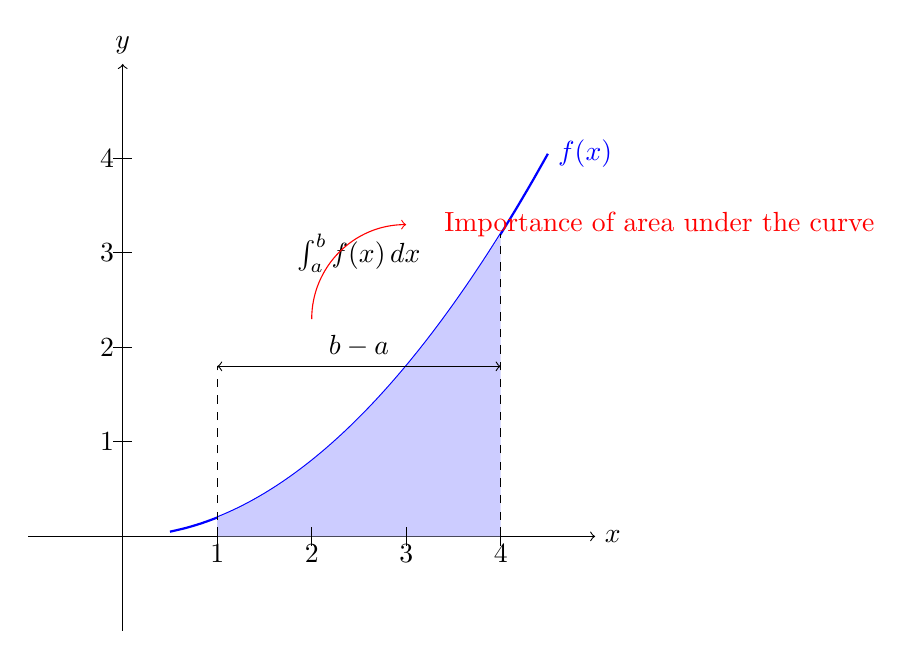
\begin{tikzpicture}[scale=1.2]
    % Axis
    \draw[->] (-1,0) -- (5,0) node[right] {$x$};
    \draw[->] (0,-1) -- (0,5) node[above] {$y$};
    
    % Function
    \draw[thick, domain=0.5:4.5, smooth, variable=\x, blue] plot ({\x}, {0.2*\x*\x}) node[right] {$f(x)$};
    
    % Integral area
    \fill[blue!20] (1,0) -- plot[domain=1:4, smooth, variable=\x] ({\x}, {0.2*\x*\x}) -- (4,0) -- cycle;
    
    % Axis labels
    \foreach \x in {1,2,3,4}
      \draw (\x,-0.1) -- (\x,0.1) node[below=3pt] {\x};
    \foreach \y in {1,2,3,4}
      \draw (-0.1,\y) -- (0.1,\y) node[left=3pt] {\y};
    
    % Integral notation
    \draw (2.5,3) node {$\int_a^b f(x) \, dx$};
    \draw[dashed] (1,0) -- (1,1.8) (4,0) -- (4,3.2);
    \draw[<->] (1,1.8) -- (4,1.8) node[midway, above] {$b-a$};
    
    % Importance of area
    \draw[red,->] (2,2.3) to [out=90, in=180] (3,3.3);
    \draw[red] (3.3,3.3) node[right] {Importance of area under the curve};
  \end{tikzpicture}
  \caption{Importance of Area under the Curve}
\end{figure}

\end{document}
